\documentclass[master]{subfiles}
\begin{document}
\section{Introduction}
\subsection{TORCS, Direct Perception, and Recurrency}
As discussed in Part 1, \cite{deepdriving} showed the feasibility of the direct perception paradigm as applied to a TORCS driving dataset.  We then showed that implementing a recurrency within the data model offered predictive benefits, through a series of rigorous statistical analyses.  The next step, then, is to build a recurrent model using state-of-the-art methods, and evaluate it on the TORCS dataset.  To do this, we look to deep artificial neural networks, which have recently gained traction as the industry standard in machine leraning models.\par
While \cite{lenet} and many others have shown that convolutional neural networks (CNNs or convnets) have provided massive performance gains in image recognition, recurrent neural networks (RNNs) have proved very useful for temporal and sequential data.  The idea behind RNNs simply relies on activation and excitation of neuron layers without external inputs -- in other words, connections between units can form directed cycles, allowing for the network to exhibit dynamic and temporal behavioral qualities.  Most practical applications of RNNs use a special network structure called Long Short-Term memory, or LSTM networks.\par
LSTM networks have recently experienced a resurgence within machine learning applications -- Google, for example, has LSTM implementations powering parts of Google Brain, applied to voice and facial recognition.  LSTMs were first developed and analyzed in 1997, by \cite{lstm_hochreiter}.  Previous work by \cite{hochreiter_analysis} showed that in training previous recurrent models, error signals flowing backwards in time either blew up or vanished.  In the first case, weights would oscillate without convergence, and in the second, the network would be unable to learn to bridge the long time lags effectively.  \cite{lstm_hochreiter} proposed LSTM as a recurrent network architecture designed to overcome error-flow problems, and bridge long time intervals despite noise issues.  After introducing the architecture, they conducted a series of experiments that showed the consistent high performance of LSTM models in long minimal time lag data.  For the experiments, they selected arbitrary LSTM architecture (single memory cell, two memory cells, etc.) and compared them to baseline RNNs, such as RTRL (Real-Time Recurrent Learning) and BPTT (Back-Propagation Through Time).  Empirical evaluation in these experiments demonstrated the potential of LSTM models in machine learning efforts.
\subsection{LSTM in Caffe}
\cite{lrcn2014} proposed a Long-Term Recurrent Convolutional Network (LRCN) that combines the strength of CNNs in visual recognition problems with stacked LSTM modules for image description tasks.  They demonstrated the viability of this approach through empirical evaluation, and were generous enough to provide a pull request to the official Caffe repository adding support for RNNs and LSTMs.  \cite{chenyi_phd} then adapted their LSTM and RNN layer implementations to the TORCS data from \cite{deepdriving} and Part 1 of this thesis, creating multiple model structures implementing a recurrency.  For our nonparametric extension, we choose one of said pipelines.  The structure is included in Figure \ref{fig:chenyi_lstm}, courtesy of \cite{chenyi_phd}.
\begin{landscape}
 \begin{figure}
  \centering
  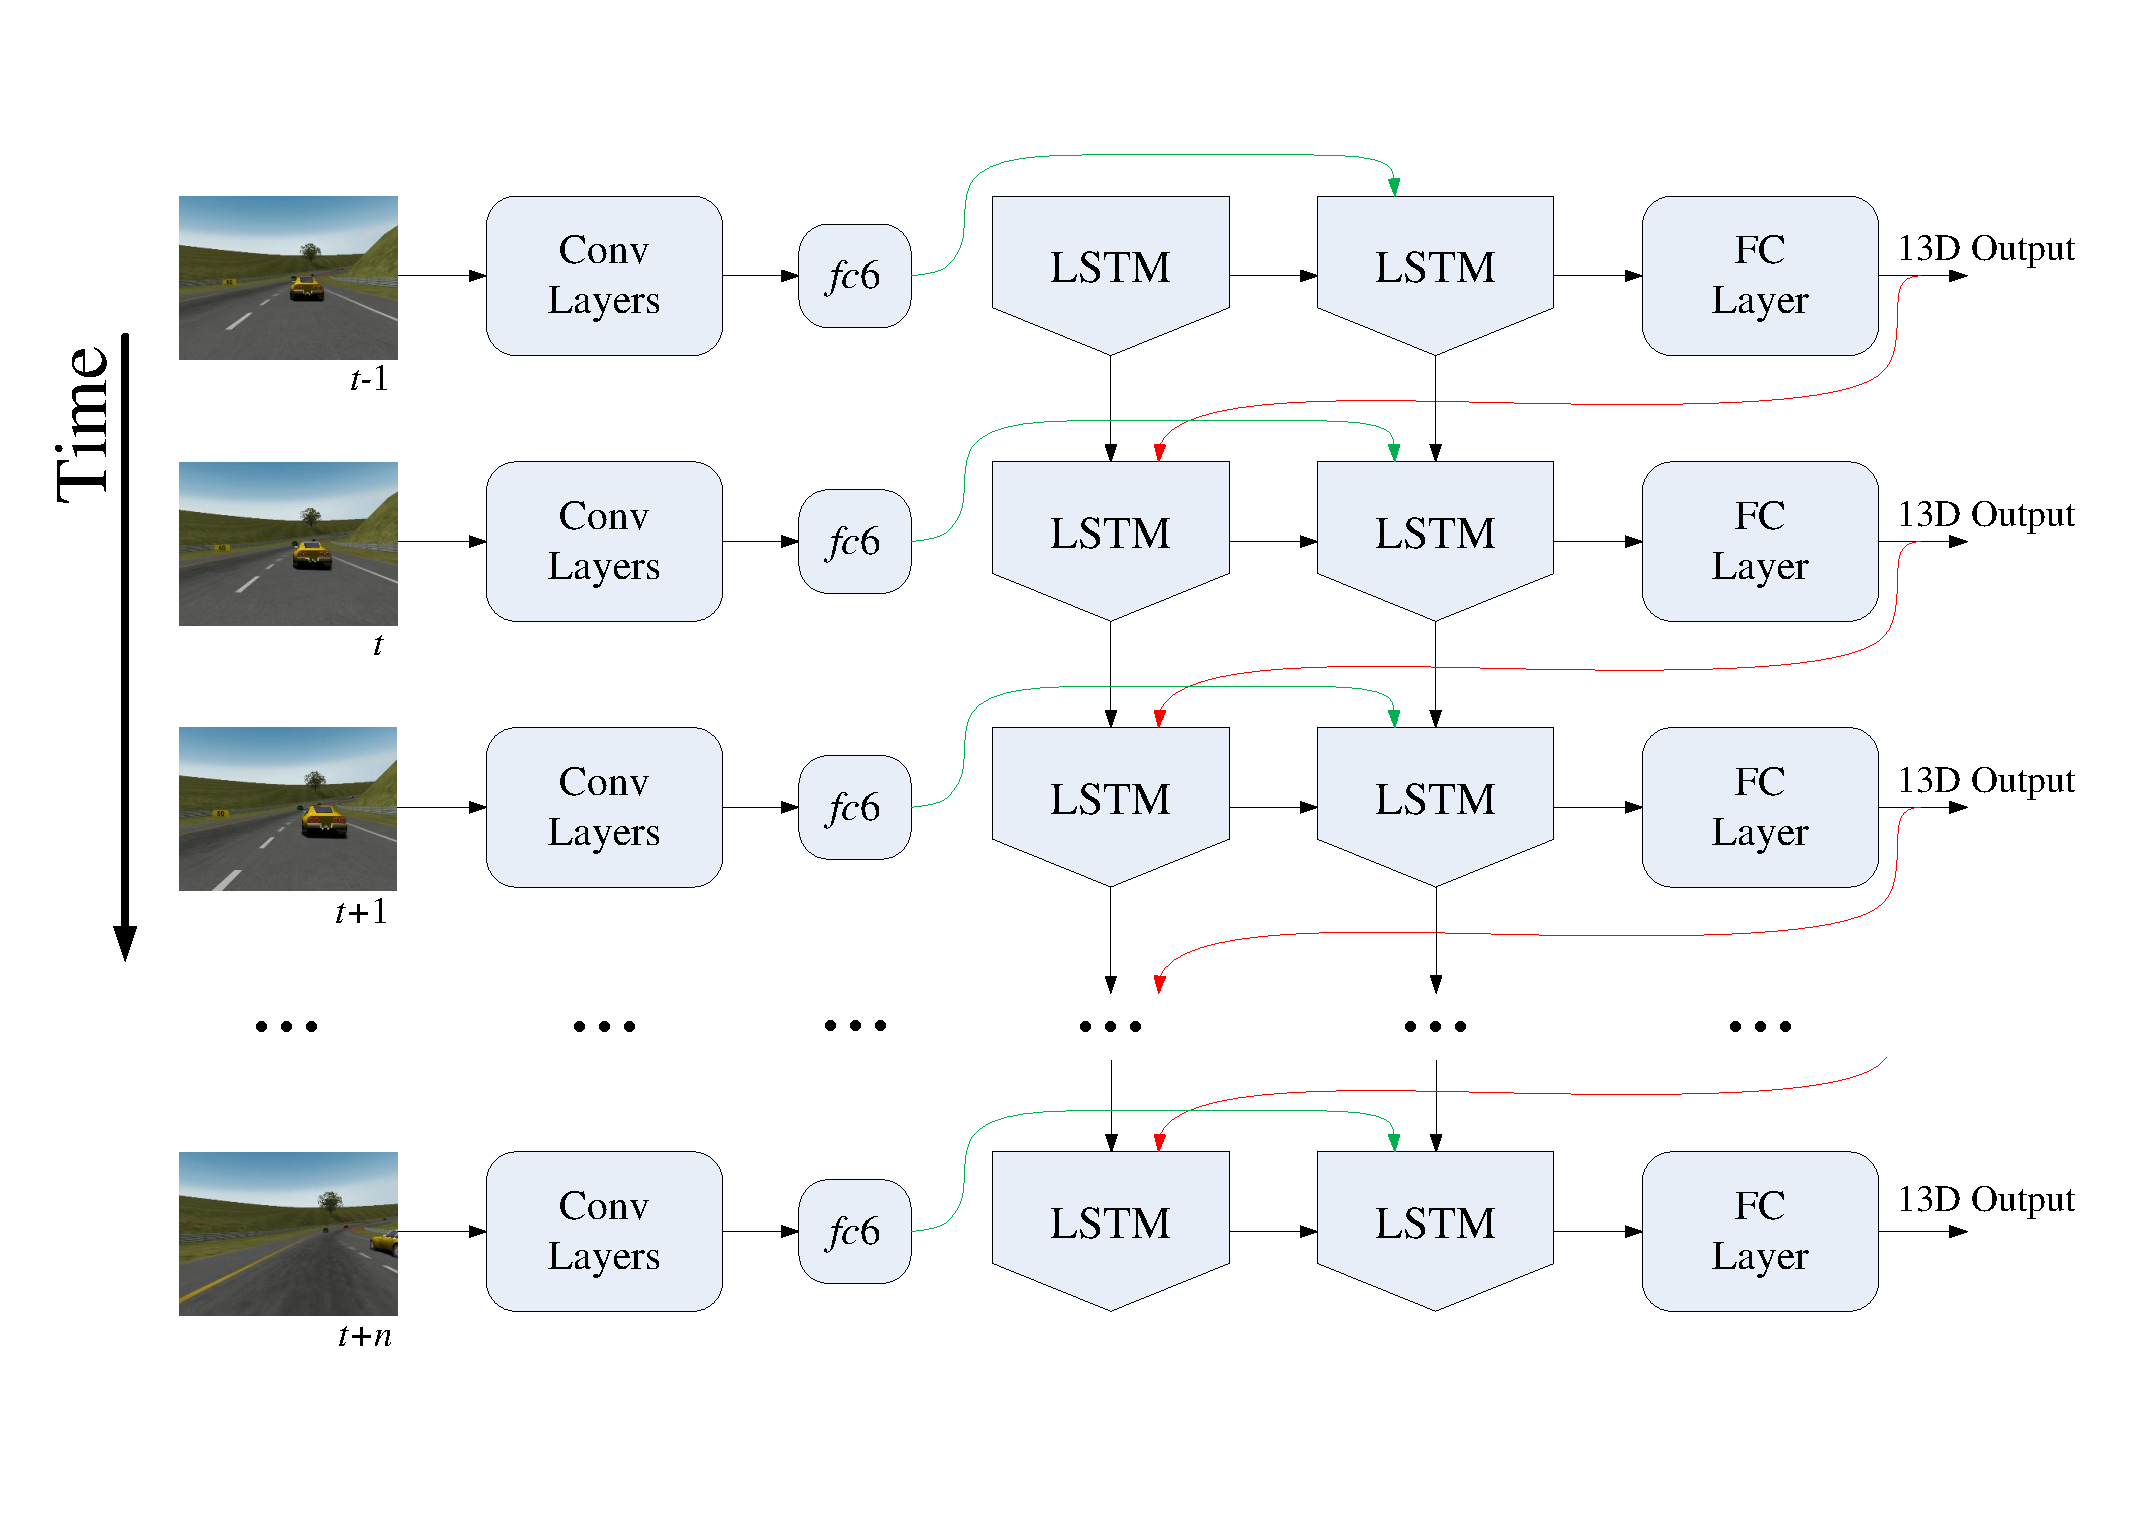
\includegraphics[width=\linewidth]{figs/LSTM_2layer_FB_skip.pdf}
  \caption{Chen's TORCS 2-Layer Skipped LSTM Structure.  Images are fed into convolutional layers, followed by a fully connected activation.  These, in turn, feed into the second of two LSTM modules (LSTM 2), as does the first of the LSTM modules (LSTM 1) and the LSTM 2 of the previous time step.  LSTM 1 also receives input from the LSTM 1 and the affordance indicator output at the previous time step.  LSTM 2 is then followed by another fully connected layer, which produces the final output response, the 13 affordance indicators.  Note that in Part 1, a 14th response variable pointing to TORCS video clip endings was used, but it is omitted in the output of this model.}
  \label{fig:chenyi_lstm}
 \end{figure}
\end{landscape}
\section{Methods}
\subsection{Nonparametric ReLU}
As is standard within deep neural networks, there are activation layers surrounding fully connected and other layer types in the LSTM network structure of \cite{chenyi_phd}.  The function of these layers can be abstractly thought of as the firing of neurons within the brain.  Popular activation functions include the sigmoid, softmax, and rectified linear unit (ReLU) functions.  The LSTM network structure we use largely contains ReLU layers for activation.\par
We look to implement nonparametric basis extensions for these ReLU layers, and examine the performance of the modified network.  As proposed by Prof. Liu, the addition of nonparametric bases into deep neural networks increases the model exploration space.  Past work has shown that this enables the network to better capture the deep structures within the data, resulting in a more powerful model.  For the TORCS data and our selected LSTM structure, we create nonparametric versions of the ReLU layer by implementing additive factors for sigmoid and Fourier bases.  By adding these basis curves to the activation layers, we move closer to true nonparametric modeling, which is far more flexible, while still maintaining an activation function suitable for backpropagation.  The forward passes for ReLU, nonparametric sigmoid ReLU, and nonparametric Fourier ReLU are as follows:
\begin{align*}
f(\mathbf{x}) &= \max(0, \mathbf{x})\\
f_s(\mathbf{x}) &= \max(0, \mathbf{x}) + \beta_s\frac{1}{1 + e^{-\mathbf{x}}}\\
f_F(\mathbf{x}) &= \max(0, \mathbf{x}) + \beta_F^{(1)}\sin(\mathbf{x}) + \beta_F^{(2)}\cos(\mathbf{x})
\end{align*}
To implement our new layers in Caffe, we also need to specify the backward pass computation.  This pass propagates error differentials backwards from the loss at the end, allowing for each layer to update its parameters through the use of partial derivatives and the chain rule.  For our new layers, we have the partial derivatives with respect to the input and the weight parameters $\beta$:
\begin{align*}
\frac{\partial f_s}{\partial \mathbf{x}} &= \mathbbm{1}_{\mathbf{x} > 0} + \beta_s\frac{1}{1 + e^{-\mathbf{x}}}\left(1 - \frac{1}{1 + e^{-\mathbf{x}}}\right)\\
\frac{\partial f_s}{\partial \beta_s} &= \frac{1}{1 + e^{-\mathbf{x}}}\\
\frac{\partial f_F}{\partial \mathbf{x}} &= \mathbbm{1}_{\mathbf{x} > 0} + \beta_F^{(1)}\cos(\mathbf{x}) - \beta_F^{(2)}\sin(\mathbf{x})\\
\frac{\partial f_s}{\partial \beta_F^{(1)}} &= \sin(\mathbf{x}), \frac{\partial f_s}{\partial \beta_F^{(2)}} = \cos(\mathbf{x})
\end{align*}
\subsection{Parametric Initialization}
In line with past work from Prof. Liu, the training of our nonparametric deep neural network relies on a parametric initialization.  In other words, we first train the normal LSTM network structure for some number of iterations, until validation loss has converged.  Then, we initialize the nonparametric version with the parametric network's converged weights, and with all $\beta$ basis factors initialized to 0.  We then train the nonparametrically modified network for some number of iterations, until validation loss has converged.
\section{Results}
Our parametric initialization is completed after 50,000 iterations, and we re-train both sigmoid and Fourier nonparametric networks for another 50,000 iterations.  The networks are trained on 50\% of 10,000 of our TORCS images, with the other 50\% set aside for validation, using a Eucliean loss across all 13 output variables.  Figures \ref{fig:sigmoid} and \ref{fig:sincos} show the validation loss of training iteration of our two networks, and Figure \ref{fig:np_result} plots them together for comparison.
\begin{figure}[H]
\centering
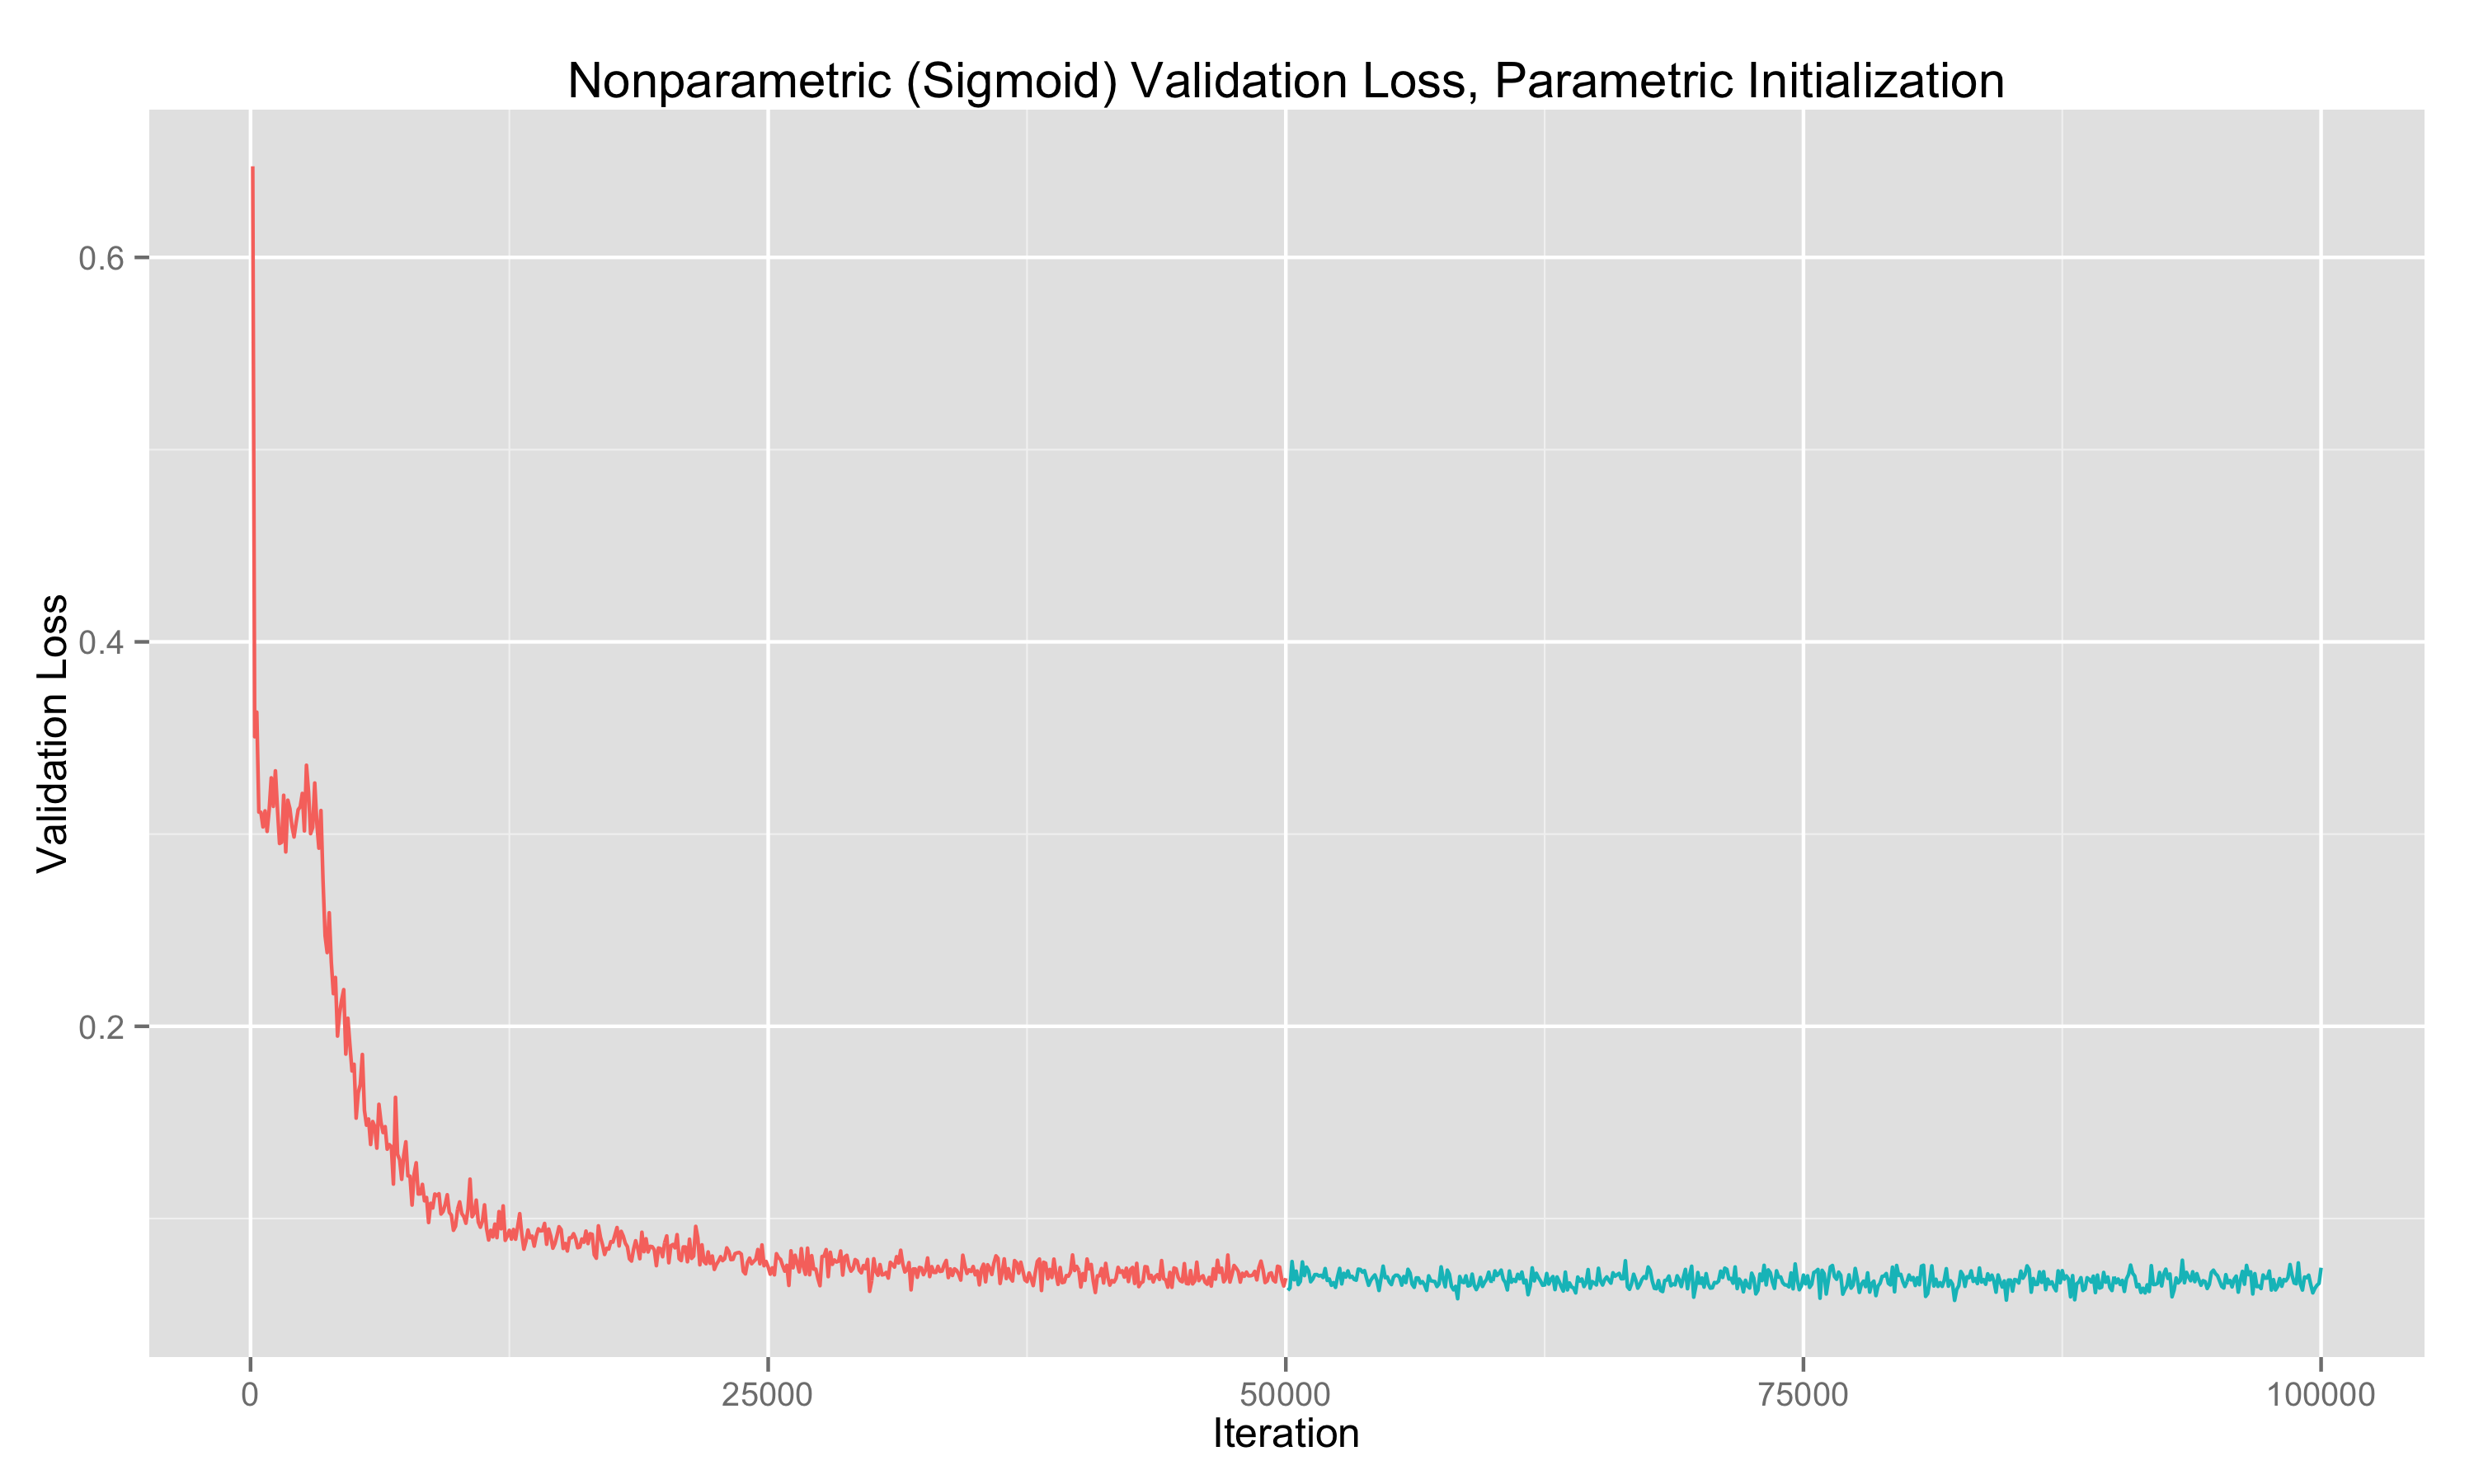
\includegraphics[width=135mm]{figs/np_sigmoid_50_init50.png}
\caption{Validation loss of the parametric and sigmoid nonparametric training.}
\label{fig:sigmoid}
\end{figure}
\begin{figure}[H]
\centering
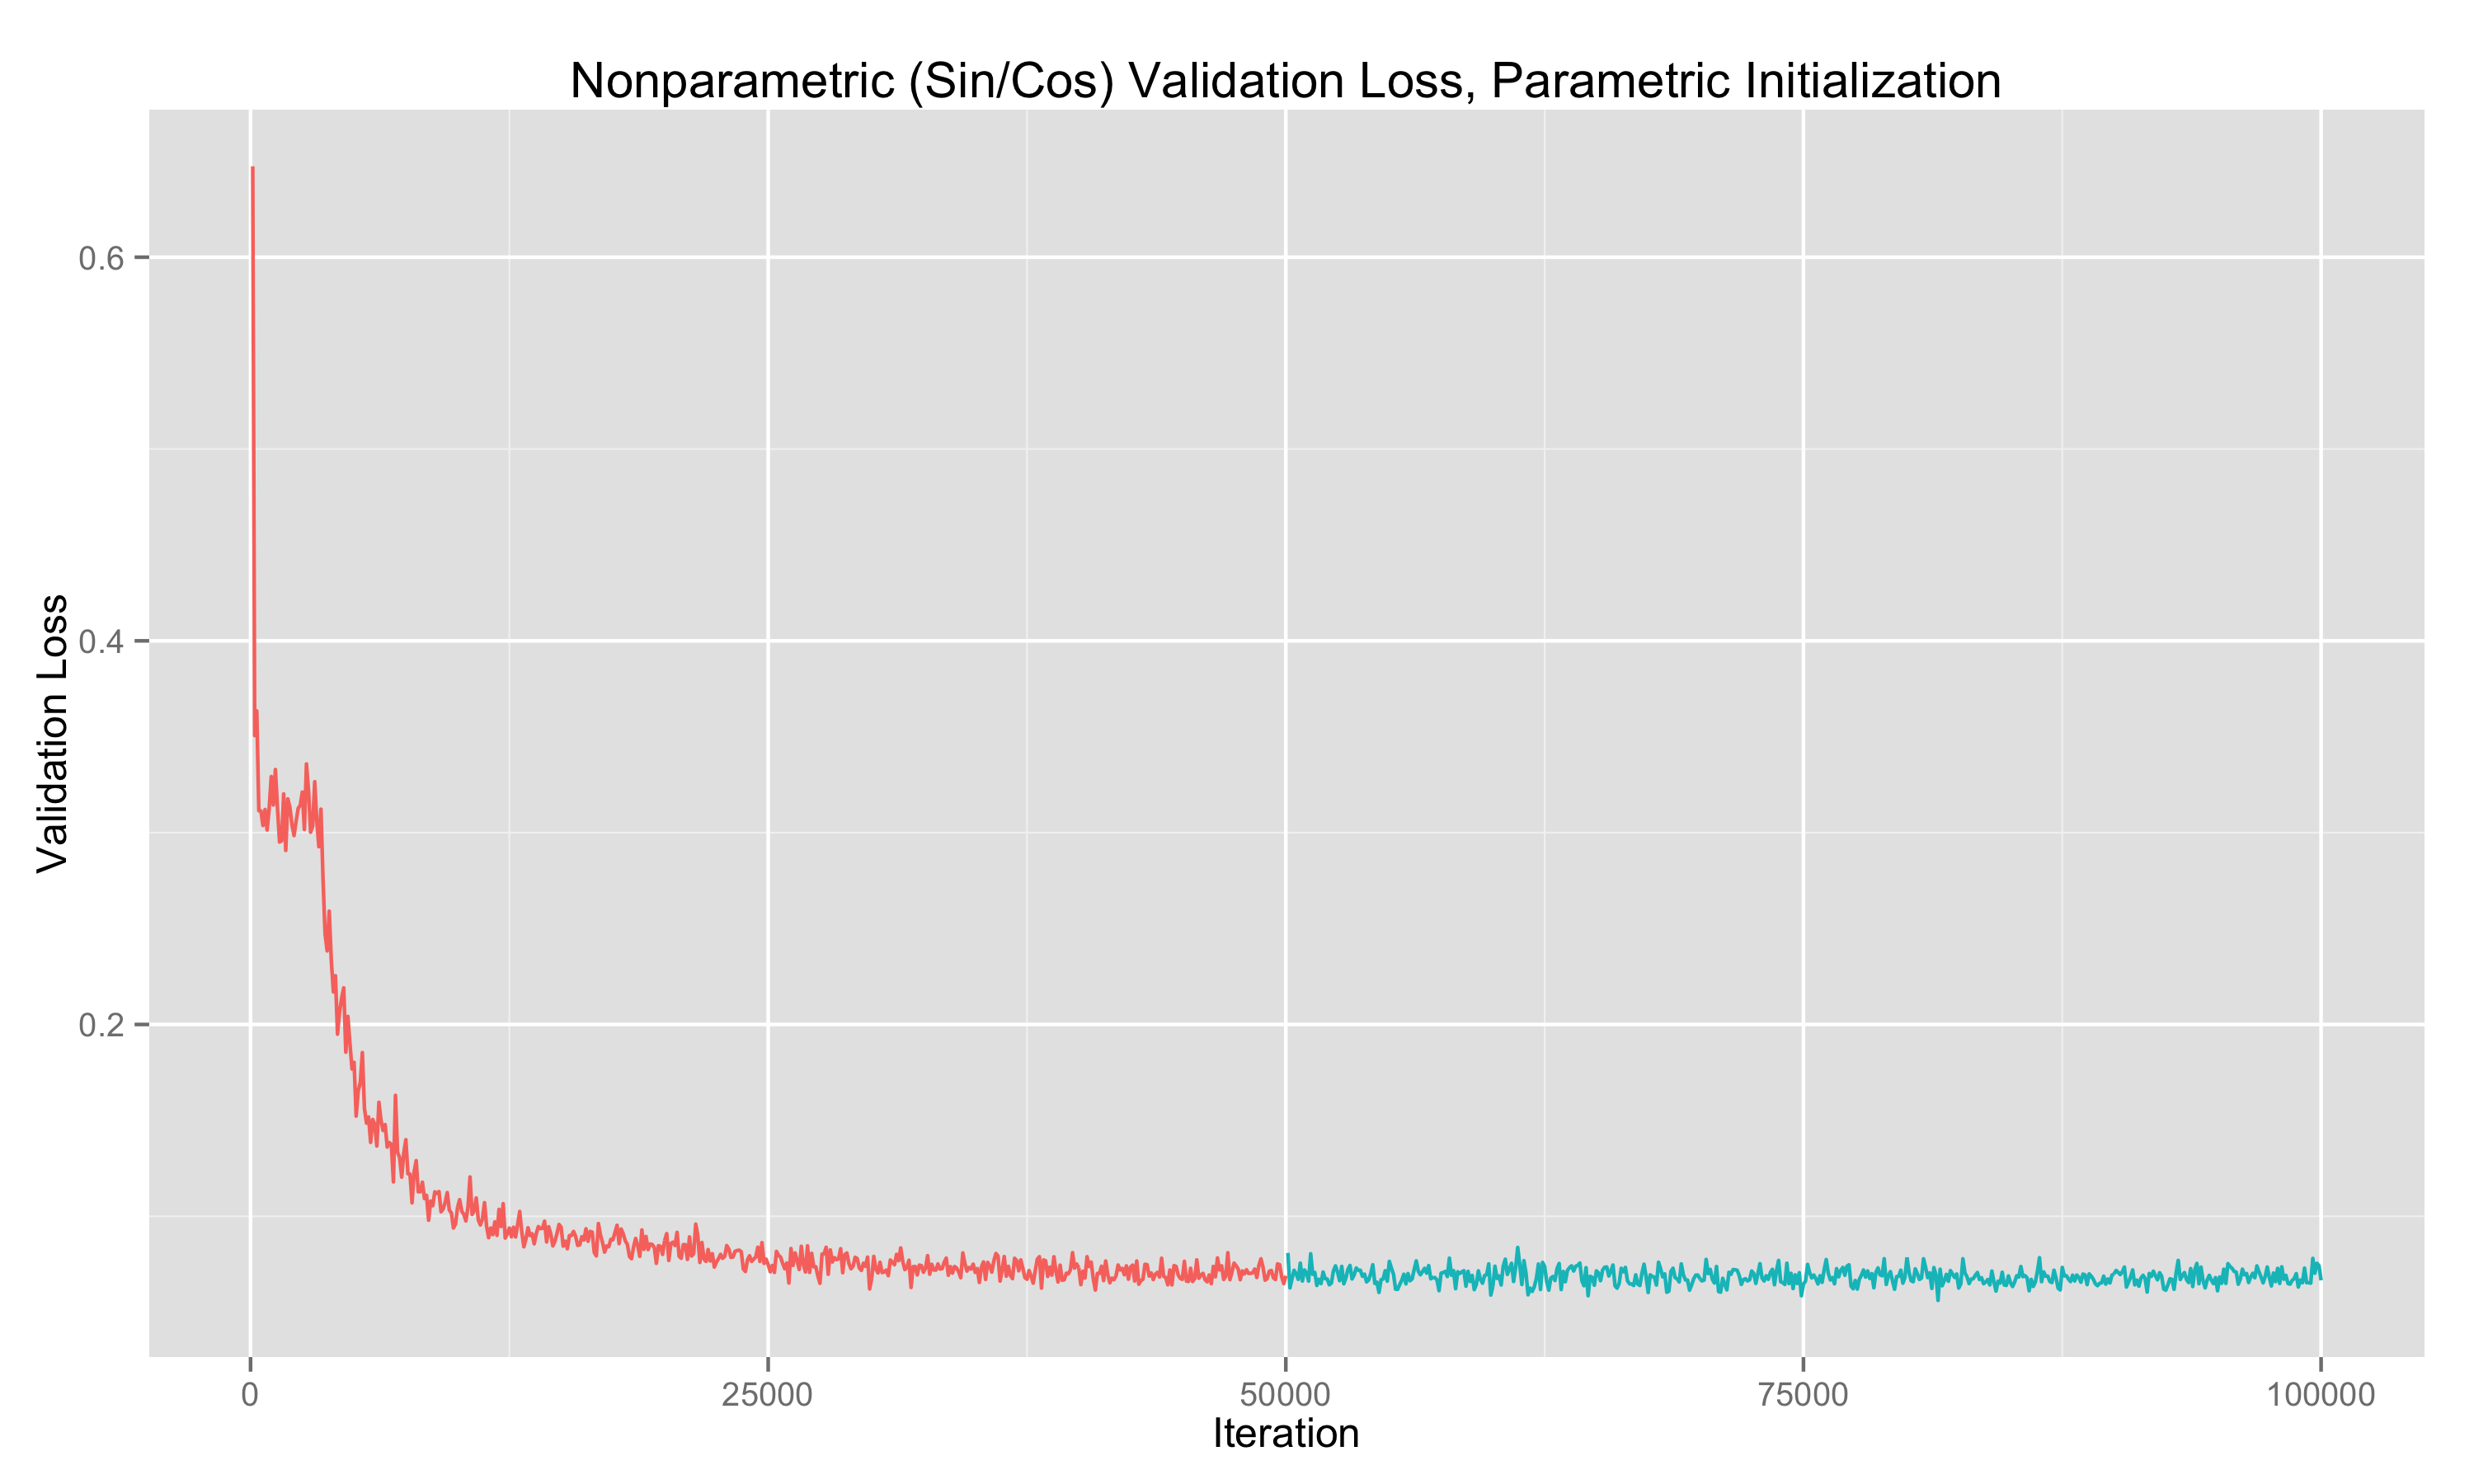
\includegraphics[width=135mm]{figs/np_sincos_50_init50.png}
\caption{Validation loss of the parametric and Fourier nonparametric training.}
\label{fig:sincos}
\end{figure}
\begin{landscape}
 \begin{figure}
  \centering
  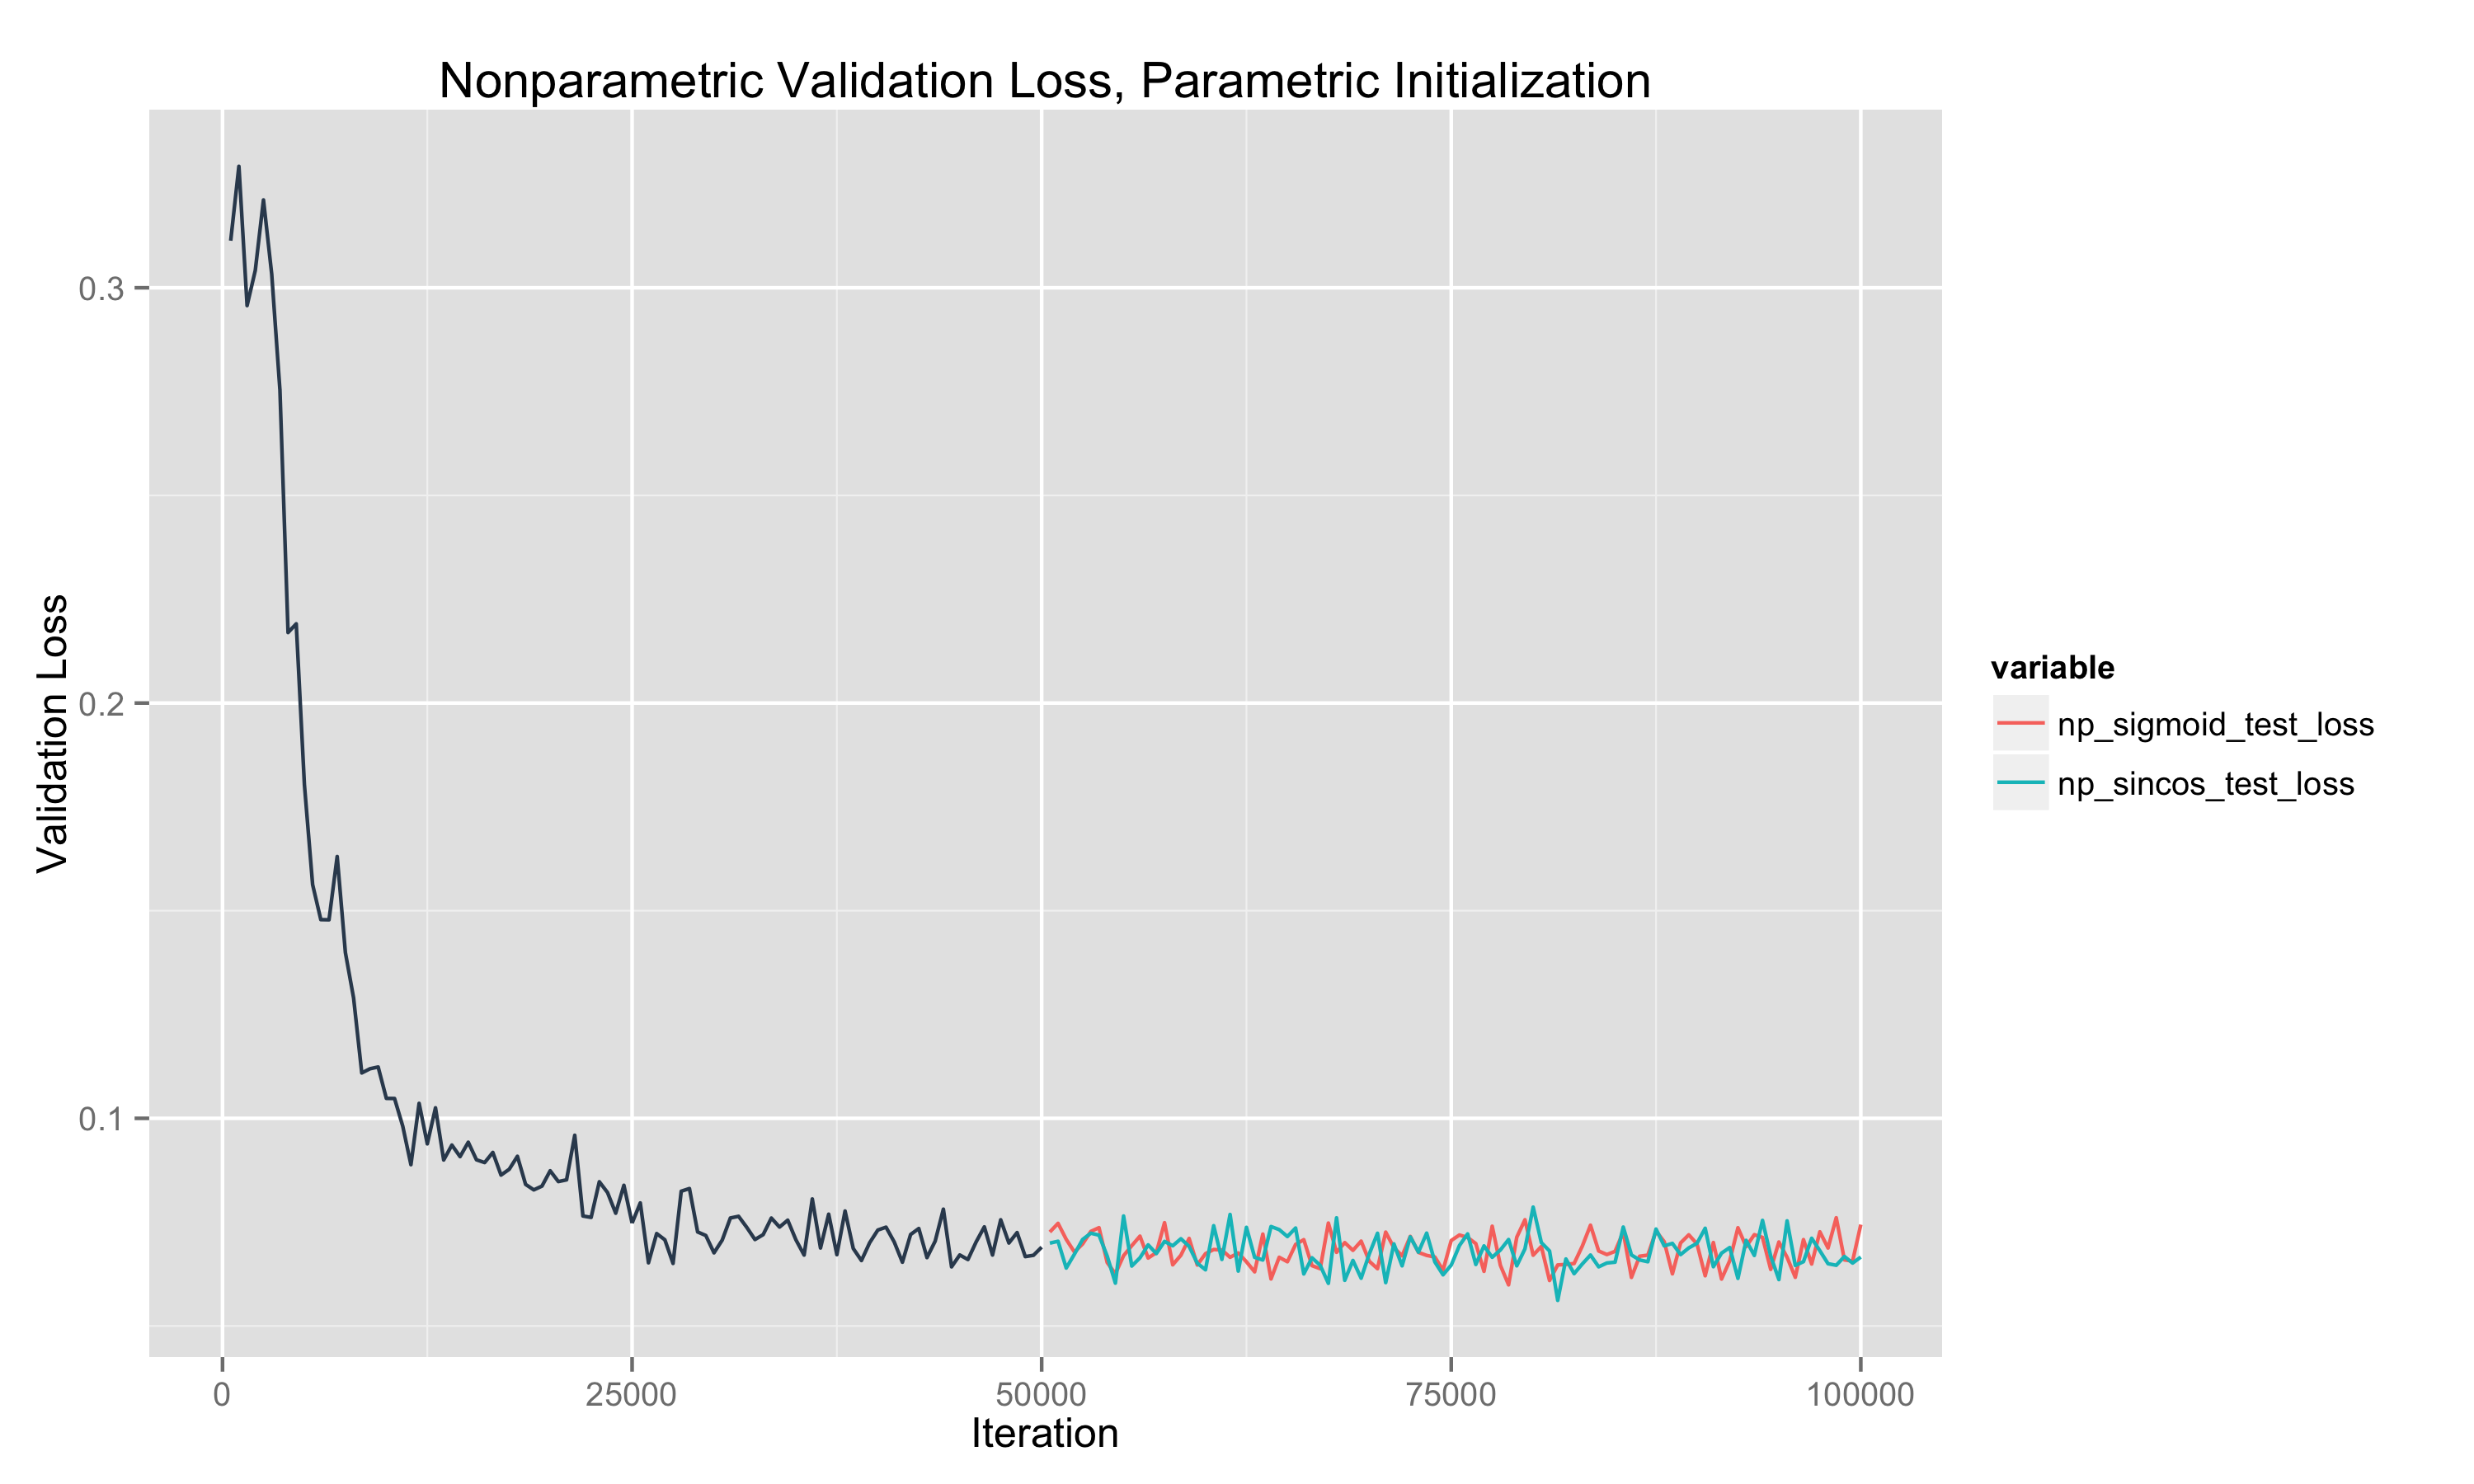
\includegraphics[width=\linewidth]{figs/np_together_50_init50.png}
\caption{Validation loss of the parametric initialization, and both sigmoid and Fourier nonparametric training.  The majority of the loss decrease is obtained during the parametric initialization, with the nonparametric networks' loss remaining around the same values as those of the parametric initialization.  Neither the sigmoid nor the Fourier-based models show stronger performance than the other, both achieving validation loss convergence at a similar level.}
 \label{fig:np_result}
 \end{figure}
\end{landscape}
\section{Discussion}
In past work by Professor Liu's group, this same methodology applied to the MNIST and other benchmark dataset showed an initial increase in loss when the nonparametric model was switched in, followed by a sharp decrease that dropped past the converged loss of the parametric initialization.  From the individual plots above, though, we see that neither our sigmoid nor Fourier basis expansions provide significant drops in validation loss -- the majority of the decrease in loss is achieved during the parametric initialization phase.   The additive nonparametric factors appear to be unable to break through the loss floor established during the initialization phase.  Moreover, the overlay plot shows that neither the sigmoid nor Fourier basis expansion achieves much lower loss than the other, so we cannot make strong conclusions comparing the validity of the two as applied to this data.  We also note that the scale of loss here is not directly comparable to that in Part 1, \textit{Nested Statistical Models}, because different magnitudes of training and validation set sizes are used.\par
As Prof. Liu notes, however, the nonparametric modified networks do not result in an overfitting and subsequent increase in validation loss, despite the largely increased model complexity.  The lack of additional loss decreases simply indicates that these nonparametric expansions are not structurally beneficial for the dataset at hand.  It is possible that other additive factors to the ReLU layers could be more suitable for the TORCS data, and enable a clear drop in validation loss.  This points to an area of further investigation:  one could explore using polynomial bases -- for example, the Lagrange or Chebyshev polynomials, which both have useful properties in interpolation and representing function spaces.  Any of these smooth functions could provide a nonparametric approximation for true structure within the data, allowing for a chance to better model the TORCS data, and subsequently, the vision-based autonomous driving problem.
\end{document}